\documentclass[10pt]{article}

% Compile from the repository root or from docs/.
% Expanded from the author draft supplied 2026-11-09.
% Figures: run scripts/build_research_report_figures.py from the repository root.
% CNN-specific passages are deliberately left pending.

% -------------------- Packages --------------------
\usepackage[margin=0.7in]{geometry}
\usepackage[T1]{fontenc}
\usepackage{amsmath,amssymb}
\usepackage{graphicx}
\usepackage{booktabs}
\usepackage{array}
\usepackage{placeins}
\usepackage{enumitem}
\usepackage[hidelinks]{hyperref}
\usepackage{titlesec}
\usepackage{parskip}
\usepackage{xcolor}

% -------------------- Formatting --------------------
\setlength{\parindent}{0pt}
\setlist[itemize]{noitemsep, topsep=3pt, leftmargin=1.5em}
\titleformat{\section}{\bfseries\large}{\thesection}{0.6em}{}
  [\vspace{-4pt}\titlerule\vspace{3pt}]
\titlespacing*{\section}{0pt}{10pt}{5pt}
\graphicspath{{docs/figures/}{figures/}{../results/}{results/}}

\newcommand{\writingprompt}[1]{\par{\small\color{gray}\textit{[Drafting prompt: #1]}}\par}
\newcommand{\cnnplaceholder}[1]{\par{\small\color{blue}\textit{[CNN pending: #1]}}\par}
\newcommand{\figureplaceholder}[1]{%
  \begin{center}
    \fbox{\begin{minipage}{0.92\linewidth}
      \centering\small\vspace{12pt}
      Figure placeholder: #1
      \vspace{12pt}
    \end{minipage}}
  \end{center}}

\title{\textbf{Predicting Maize Chromatin Accessibility from DNA Sequence}}
\author{Gregory Orme}
\date{Working draft}

\IfFileExists{linear_results_table.tex}{%
  \newcommand{\reporttablepath}{linear_results_table.tex}}{%
  \IfFileExists{docs/figures/linear_results_table.tex}{%
    \newcommand{\reporttablepath}{docs/figures/linear_results_table.tex}}{%
    \newcommand{\reporttablepath}{figures/linear_results_table.tex}}}

\begin{document}
\maketitle

\begin{abstract}
There has been extensive study of caQTLs in maize, with high-resolution mappings implicating disruption of transcription factor binding sites as a potential mechanistic avenue for differential chromatin accessibility. While caQTL studies identify specific loci associated with accessibility, the relationship between region-level sequence features and local accessibility is still unclear. In this paper, I will explore a few candidate sequence features with different levels of information to see how much certain summary statistics can predict chromatin accessibility. I compare 13 linear models on 495,900 cortex (region, genotype) observations from 9,666 accessible chromatin regions (ACRs), holding out genomic blocks for out of sample tests. The lowest observed pair RMSE is 7.556 CPM versus 7.748 for a composition/ancestry baseline, a modest 4.91\% reduction in mean squared error. SNP-substituted sequences give almost identical performance to B73 reference sequences, and genotype deviations within ACRs remain poorly predicted. I also train convolutional neural networks for the same task, whose validation performance matches the nuisance covariate baseline. Finally, I include a smaller CNN using reference sequence only which contributes an appreciable improvement over the linear models while only explaining just under a third of the variance in accessibility across ACRs.
\end{abstract}

% ==================================================
\section{Research Question}

I wanted to investigate the relationship between sequence characteristics near regulatory regions and the chromatin accessibility of those regions in the maize genome. Whereas previous studies have used QTL analysis and fine-mapping to isolate specific loci associated with chromatin accessibility, I wanted to see if there are region-level aggregate  statistics which can explain variation in accessibility at unseen ACRs. In \textit{The genetic architecture of cell type--specific cis regulation in maize}, Marand et al. profiled approximately 700,000
retained seedling nuclei from 172 inbred genotypes and annotated
33 cell populations spanning different cell identities and
developmental states~\cite{marand}. Here, I restrict the analysis
to nuclei annotated as cortex, the largest group. The authors discovered localized cell-type-specific sequence patterns associated with chromatin accessibility and implicated disruptions in TCP-family motifs as a plausible mechanism. The motif-disruption hypothesis poses an interesting question: beyond highly specific and localized disruptions to TF motifs, is average motif resemblance throughout an ACR's nearby sequence predictive of accessibility across ACRs? If average motif resemblance is predictive, how does that predictive performance compare to scoring regions against arbitrary kmers?  In either case, does including wider local sequence context improve prediction? How much does prediction improve when we represent (ACR, genotype) pairs with approximate genotype-specific sequences using a SNP panel, versus using a reference genome for all genotypes? And finally, how much better do deep learning methods perform? In this report, I investigate the feasibility of these problems, propose and test interpretable features via penalized linear regression, then compare performance with convolutional networks trained on the same dataset. 

% ==================================================
\section{Data and Processing}

\subsection{Source experiment and data resources}
In Marand et al., the authors grew seedlings from 172 inbred maize genotypes. At day 7 after germination, they collected tissue samples into 40 pooled sequencing libraries, with each genotype represented in about three pools on average. They profiled approximately 1.37 million nuclei and retained 682,794 after the study's quality-control and genotype-assignment steps~\cite{marand}. The final supplementary pool table records 493 genotype--pool memberships, or 2.87 pools per genotype, with a range of one to eight. A library contains nuclei from one or more genotypes; computational genotyping assigns each retained nucleus to a line. Pool memberships do not establish how many independent plants contributed because the supplied table does not include individual plant IDs. The plants were grown under the same intended conditions, while the 40 libraries represent separate batches processed for sequencing.

They used the aggregate Tn5 insertion profile to define 108,843 accessible chromatin regions (ACRs). For my regression formulation, I extract a sparse binary matrix whose rows are nuclei, columns are the identified ACRs, and entries indicate whether there was at least one detection in each nucleus within each ACR. The public sparse matrix used here contains binary entries, so I analyze accessibility detections as binary events within each (nucleus, ACR) pair rather than the true fragment counts which are unavailable in this matrix. I use the authors' retained nuclei and cell-state assignments without repeating their raw-read QC or peak calling. I interpret zeros as non-detections, not proof that the region was biologically closed.

To define accessibility across ACRs in genotype $g$, I restrict to cortex cells (the cell type with the most observations in the dataset), sum the binary vectors for all cells with genotype $g$, and normalize each ACR entry to a counts per million (CPM) by dividing by the total number of accessibility events within genotype $g$ and scaling by $10^6$. For the feasibility analysis, I perform this aggregation within (genotype, library) pairs to investigate the relative size of library effects versus genotype effects. This response measures relative allocation of detections across ACRs and does not represent the fraction of nuclei detecting the ACR.

To extract sequence-level features, I use the B73-v5 reference genome along with the Panzea-v5 SNP panel to construct approximate genotype-specific sequences. Notably, substituting SNPs into the reference genome is an approximation to the actual sequence of different genotypes; I did not account for indels or other non-SNP deviations from reference. The reference is \texttt{Zm-B73-REFERENCE-NAM-5.0}; the variants are the chromosome-wise, B73-v5 282-panel VCFs distributed through Panzea/MaizeGDB, derived from the HapMap resource~\cite{reference,panzea,hapmap}. To score regions against known transcription factors, I downloaded 927 plant CORE non-redundant PFMs from JASPAR 2026 and converted them to probability matrices via a convex combination with a uniform background distribution~\cite{jaspar}.

I wanted to control for population structure when predicting accessibility and used ten principal components from the separate TASSEL tutorial marker panel, \texttt{mdp\_genotype.hmp.txt}, as population proxies~\cite{tassel}. This compact panel has 3,093 markers across 281 inbred lines. The inherited preprocessing parses biallelic dosages, removes entirely missing markers, mean-imputes missing calls, removes invariant markers, standardizes each marker, and retains ten PCs from the resulting 2,907 variable markers. PCA was computed on the full 281-line marker panel, then rows were explicitly aligned to our development genotypes. The PCs and loadings are static throughout the regression process; I do not refit them within training folds of regression or the CNN. They do not represent a complete correction for relatedness or substitute for a genome-wide SNP prediction baseline.


\subsection{Accessibility response and notation}

Let $i$ and $j$ index ACRs, $g$ index genotypes, $\ell$ index sequencing libraries, $m$ index TF motifs or 5-mer features, $k$ index ancestry principal components, $r$ index a sequence placement, and $s$ index DNA orientation. For the cortex nuclei assigned to genotype $g$ in library $\ell$, let $N_{g\ell}$ be the total number of nuclei and define
\[
Y_{ig\ell}=\sum_{n=1}^{N_{g\ell}}\mathbf{1}\{\text{nucleus }n\text{ detects ACR }i\},
\qquad
T_{g\ell}=\sum_{j=1}^{108843}Y_{jg\ell}.
\]
So $Y_{ig\ell}$ counts total nuclei detecting ACR $i$ within the $(g, \ell)$ stratum, while $T_{g\ell}$ counts all detections over the entire set of ACRs in those same cortex nuclei (and same $(g, \ell)$ stratum). A nucleus can contribute to multiple ACRs, so $T_{g\ell}$ is not a cell count. 
\begin{equation}\label{eq:response}
C_{ig}=10^6\frac{\sum_{\ell}Y_{ig\ell}}{\sum_{\ell}T_{g\ell}}.
\end{equation}
$T_{g\ell}$ aggregates accessibility counts within (genotype, library) pairs, while $C_{ig}$ is the CPM of observations in ACR $i$ out of all ACRs in genotype $g$. In this analysis, $C_{ig}$ defines the target of prediction. Libraries are pooled within genotype by summing counts before dividing, while genotypes remain separate observations. The denominator always uses all 108,843 ACRs, including regions outside the sampled prediction set. The target remains the original ACR's CPM when I enlarge the sequence input to 2,000 bp. I do not log-transform, rank-transform, or clip this response.

\subsection{Genotype-specific sequence construction}
To construct genotype-specific sequences, I use the B73 reference genome along with a panel of SNPs. Genotypes which are heterozygous at a SNP introduce uncertainty about representing their sequence, so I restrict the prediction task to (ACR, genotype) pairs for which the 2,000-bp total window centered on the ACR contains only complete homozygous calls at every listed biallelic SNP. This omission is for practical ease and represents a notable limitation, along with the fact that I am substituting SNPs into a reference genome to arrive at the genotype-specific sequences (and hence ignoring indels and other variations). My goal is not to fully represent every genotype within every ACR, since the data is already large enough that I sample ACRs to train on my computer and retain all usable genotypes at each sampled ACR. Even so, the restriction to regions containing only homozygous SNPs is a bias which means these predictive results may not generalize to heterozygous loci or to the true genotype-specific sequences. Additionally, I should note that the Panzea-v5 SNP panel is not an exhaustive list of SNPs and there is uncertainty about the true values which I am not accounting for in this analysis. At a listed SNP, a $0/0$ call retains the B73 base and a $1/1$ call substitutes the alternate base. A missing or heterozygous call makes that (ACR, genotype) pair unavailable; it is not filled with B73. I checked that every listed SNP’s reference base matched B73 at the corresponding position. The downloaded SNP files did not include read depth or confidence scores for individual genotype calls, so I could not filter calls using those measures.

I call the original variable-width ACR the \emph{core} and the entire midpoint-centered 2,000-bp sequence the \emph{full window}. This means roughly $\pm 1,000$ bp from the midpoint, not an extra 1,000 bp on either side of each ACR boundary. Shorter cores therefore receive more padding sequence. 

I compare all models in this matched experiment using exactly the same ACR–genotype observations and training/validation splits. An observation is included only if its full 2,000-bp sequence can be reconstructed with nonmissing, homozygous calls at every SNP listed in the panel, even when the model uses only the ACR sequence itself (unpadded) or the B73 reference. 

For cross-validation, I group nearby ACRs into chromosome-specific 5-Mb blocks and keep each block entirely in training or validation. Sequence windows may overlap within a block, but I exclude windows that would extend across the boundaries separating blocks or beyond a chromosome end. This prevents training and validation inputs from sharing DNA. Every retained window includes the entire original ACR. 

% ==================================================
\section{Measurement Quality and Dataset Eligibility}

\subsection{Variation across genotypes and libraries}
Recall that single cell observations vary across cell type, genotype, and sequencing library. The objective $C_{ig}$ sums accessibility events across libraries and represents an estimated CPM of accessibility events from ACR $i$ in genotype $g$. Sequencing noise can be quite large, so before asking if genotype-specific sequences are relevant for accessibility, we should check how much mean accessibility varies between genotypes (pooling libraries) versus within genotypes (separating libraries) at different ACRs.

Let $G$ = 138 (the 138 development genotypes). At a fixed ACR $i$, define the library CPM, total-detection weight, and average genotype CPM (respectively) as
\[
R_{ig\ell}=10^6Y_{ig\ell}/T_{g\ell},\qquad
w_{g\ell}=\frac{T_{g\ell}}{\sum_{\ell'}T_{g\ell'}},\qquad
\bar C_i=\frac{1}{G}\sum_g C_{ig}.
\]
The weighted library mean is exactly the pooled CPM: $C_{ig}=\sum_\ell w_{g\ell}R_{ig\ell}$. I compare
\begin{align}
V_{\mathrm{library},i}&=\frac{1}{G}\sum_g\sum_\ell w_{g\ell}(R_{ig\ell}-C_{ig})^2,\label{eq:libraryvar}\\
V_{\mathrm{genotype},i}&=\frac{1}{G}\sum_g(C_{ig}-\bar C_i)^2.\label{eq:genotypevar}
\end{align}
The first quantity averages squared library deviations from each genotype's pooled CPM; the second measures variation among those pooled genotype CPMs. Genotypes have equal weight, while libraries within a genotype are weighted by total detections, not nucleus counts. Both the library and genotype variances are in CPM$^2$ and use population denominators $G$, without a degrees-of-freedom correction. Their sum is the total observed CPM variance under these weights. I pursue this  descriptive comparison instead of a formal F-test due to multiple likely violations of the F-test assumptions which would make the conclusions misleading. I've listed a formal statistical investigation of these effects as one of my potential future directions. 

This diagnostic uses all 108,843 ACRs and 138 development genotypes, including H95, which is excluded from model training due to small nuclei counts. We have 93,651 cortex nuclei in 384 observed genotype/library groups to run the diagnostic. Mean library variance is 55.887 CPM$^2$, versus 37.02 for genotype means; the corresponding medians are 40.13 and 30.91. Library variance exceeds genotype-mean variance at 77.03\% of ACRs (Figure~\ref{fig:variance}). Seven genotypes have only one cortex library and therefore contribute zero observed within-genotype library deviation. Restricting both quantities to the 131 genotypes with multiple libraries gives means of 58.873 versus 34.380 CPM$^2$, with larger library variance at 86.72\% of ACRs.

Most ACRs therefore show substantial library-to-library variation relative to the spread of pooled genotype means. This is another notable limitation of this analysis which suggests we may not be able to reliably estimate how sequence-level features contribute to varying accessibility across genotypes within ACRs. However, these calculations describe the observed CPM differences without identifying their causes. Differences between libraries may reflect limited sampling of nuclei, experimental preparation, or biological differences between samples. Pooled genotype CPMs retain some of this uncertainty, although combining libraries generally reduces sampling fluctuations. We therefore cannot interpret the two quantities as separate estimates of genetic variance and technical noise. In the analysis, I test the predictive power of using the genotype-specific sequences versus imposing the reference sequence on all genotypes. I use within-ACR $R^2$ to assess whether genotype-specific
sequences improve prediction of differences between genotypes
within the same ACR; overall RMSE mixes predictive accuracy within ACRs with prediction of
differences between ACRs. If genotype-specific sequence models cannot explain variation in accessibility within ACRs, this failure might be due to model limitations and does not rule out genotype-specific variation. 

\begin{figure}[htbp]
\centering
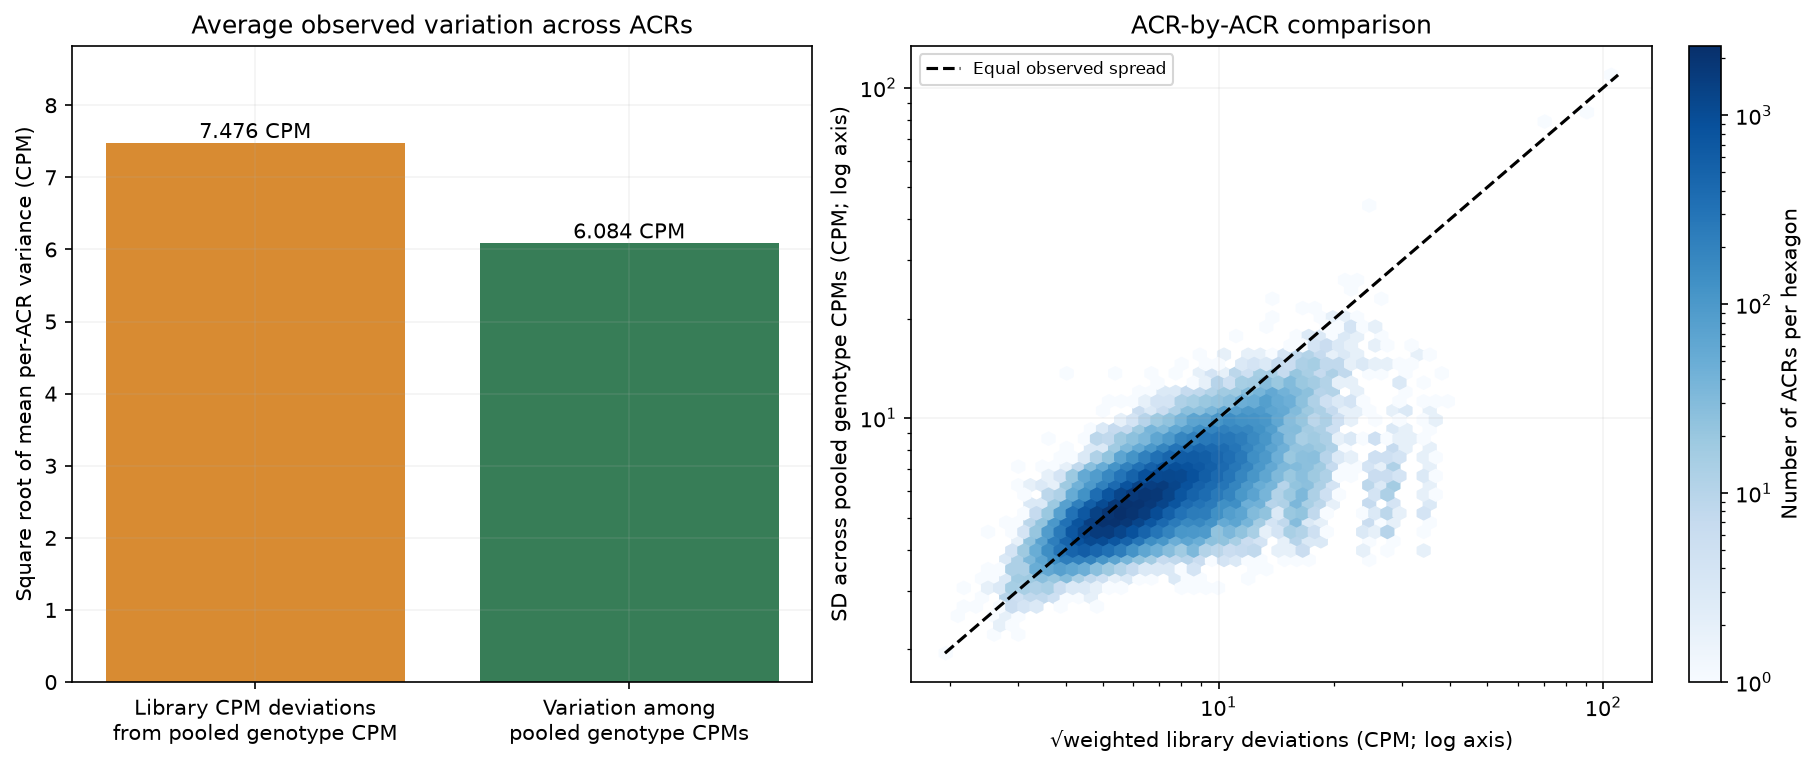
\includegraphics[width=\linewidth]{cortex_cpm_variance.png}
\caption{Observed cortex CPM variation across all 108,843 ACRs and 138 development genotypes. Left: square root of the mean per-ACR variance, not the mean per-ACR standard deviation. Right: hexagon density of individual ACRs, comparing $\sqrt{V_{\mathrm{library},i}}$ with $\sqrt{V_{\mathrm{genotype},i}}$. Both axes are logarithmic; the dashed line marks equality. Counts, weights, and variances are defined in Equations~\ref{eq:response}--\ref{eq:genotypevar}. No ACRs have a zero on either plotted axis. These are observed spreads and not proper estimates of genetic and technical variance components.}
\label{fig:variance}
\end{figure}

\subsection{SNP completeness and spatial sampling}

The starting cohort comprised 169 lines retained during an earlier alignment of accessibility and phenotype datasets. I preserved this cohort for consistency across experiments, and phenotype values were not used in the accessibility-prediction models. I reserve a permanent 30-genotype holdout from those 169 genotypes for use in future analyses. Those 30 are not used at all in this paper. I subsequently remove CML341 from the development cohort because of accessibility quality control: 69.6\% of ACRs contain zero detections, there are only 495 assigned cells, and CML341's unusual observations exert strong influence on accessibility PCA. The holdout set is not regenerated after this exclusion, leaving 138 development genotypes. I further enforce that each line must have at least 50 observed nuclei among cortex cells, which excludes H95 (49 nuclei), leaving us with 137 prediction genotypes. 

I then remove (genotype, ACR) pairs with missing or heterozygous calls at any listed SNP within the full 2,000-bp window and require unambiguous, unclipped reference sequence. An eligible ACR must contribute at least 20 genotypes matching these restrictions. Among 108,843 candidate ACRs, 19,201 remain. After fixing random seed 42, I sample up to 25 ACRs from each of the 432 occupied chromosome-specific 5-Mb blocks, yielding 9,666 ACRs and 495,900 (genotype, ACR) pairs covering all ten chromosomes of the B73 reference (Figure~\ref{fig:funnel}). All available genotypes at each sampled ACR are retained, and all 137 development genotypes are represented, with 1,808--7,949 observations each.

If block $b$ contains $N_b$ eligible ACRs, each has inclusion probability $\pi_i=\min(1,25/N_b)$. As a result, the sample favors spatial coverage over uniform inclusion across all eligible ACRs. I save these probabilities but weight the retained observations equally irrespective of their sampling probabilities. Additionally, I do not apply any filters for accessibility, minor allele fraction, SNP count, or other characteristics. In particular, 1,755 sampled windows contain no listed SNPs; their completeness requirement is vacuous and does not demonstrate that their real sequences are identical across genotypes.

Among the selected ACRs, I annotate a \emph{core-variation-rich} subgroup when at least two distinct core sequences are each represented by five or more usable genotypes. This gives 2,167 ACRs and 70,594 pairs. Applying the same rule to the entire 2,000-bp sequence gives a \emph{context-variation-rich} subgroup of 4,305 ACRs and 154,395 pairs. To examine whether personalization helps at regions with common sequence variation, I separately summarize prediction performance for these two ACR subsets. Both classifications use only genotypes with reconstructable full windows. An ACR can qualify for either subset or both. These classifications do not change the main sample or model fits. Each subset includes all usable genotypes at its qualifying ACRs.

\begin{figure}[htbp]
\centering
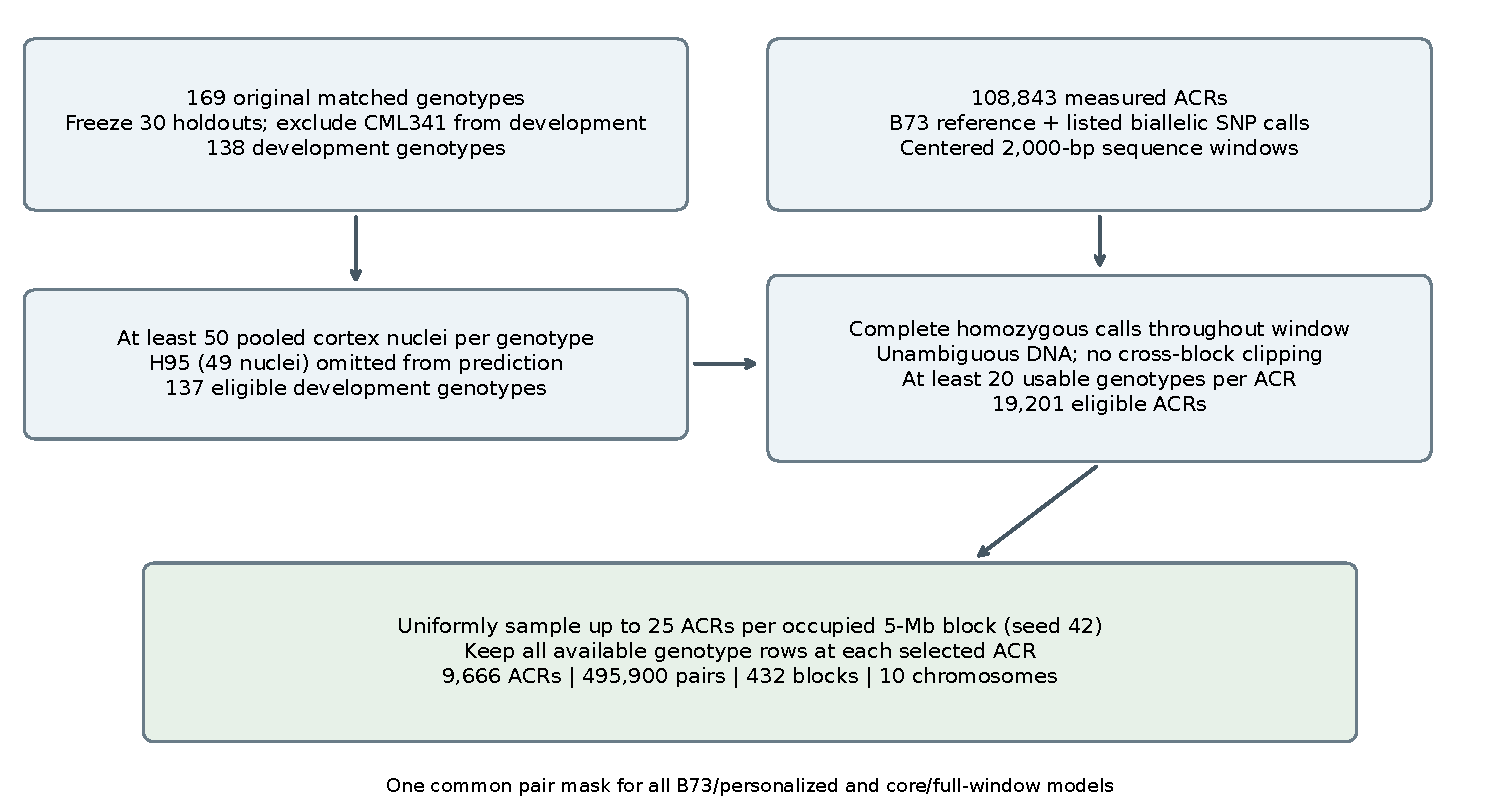
\includegraphics[width=0.98\linewidth]{sampling_funnel.pdf}
\caption{Outcome-independent eligibility and sampling. The genotype and ACR restrictions intersect to produce the common matched pair set used by all 13 models. ACRs are sampled first, with all their usable genotypes retained. Five-Mb blocks organize sampling and cross-validation and do not impose any further biological aggregation of ACRs.}
\label{fig:funnel}
\end{figure}
\FloatBarrier

% ==================================================
\section{Models and Evaluation}

\subsection{TF motifs and 5-mer quasi-motifs}
Position-frequency matrices summarize nucleotide frequencies at sites associated with a transcription factor. The PWM model treats positions as independent and defines probabilities under a motif model, rather than directly measuring the probability that a TF is bound in these maize cortex nuclei. To convert a PFM to a matrix of probabilities, I normalize its columns and take the convex combination of $99\%$ of the original probabilities and $1\%$ of an even-probability matrix. This mixing prevents individual entries from equaling zero, thereby avoiding undefined log probabilities. If $F_{mab}$ is the frequency count for base $b$ at motif position $a$, then
\[
P_{ma}(b)=0.99\frac{F_{mab}}{\sum_{b'}F_{mab'}}+0.01\times\frac14.
\]
In an ideal world, a calibrated binding model could help calculate a posterior probability $P(\text{TF bound}\mid\text{sequence})$. However, motif probabilities alone do not supply the necessary priors, cellular context, or occupancy model. I choose instead to use a likelihood-ratio proxy comparing the motif model with an independent, uniform-nucleotide background. Taking the log of that ratio provides a score for each potential binding site and gives us a rough sense for how plausible that sequence would be under the motif model. Importantly, this score is not direct evidence of binding and should not be interpreted as such. Rather, my hypothesis is that if certain classes of TF motifs are associated with looser chromatin (either by acting as pioneers or by opportunistically binding in open regions), then perhaps regions with higher resemblance to those motifs are systematically more accessible.

I downloaded 927 TF PFMs from JASPAR, converted them to probability matrices using the smoothing method described above, and scored the sequences associated with all 495,900 (genotype, ACR) pairs using this formula. 

Fix an ACR $i$, genotype $g$, and motif $m$, and choose either the core
sequence or the full 2,000-bp sequence for that pair. Let $w_m$ be the
motif's width in bases. For motif position $a=1,\ldots,w_m$, let
$P_{ma}(b)$ denote the smoothed motif probability assigned to nucleotide
$b\in\{A,C,G,T\}$ at that position.

Let $\mathcal R_{igm}$ contain all starting positions where the entire
motif fits within the chosen sequence. Its size, $|\mathcal R_{igm}|$,
is the number of valid placements. For an unambiguous sequence of
length $n_{ig}$, this number is $n_{ig}-w_m+1$.

I scan both the forward sequence ($s=+$) and its reverse complement
($s=-$). Let $B_{igrsa}$ be the nucleotide at motif position $a$ when
starting at position $r$ in orientation $s$. Thus,
$P_{ma}(B_{igrsa})$ is the probability that the motif assigns to the
nucleotide actually observed there. The background assigns probability
$1/4$ to each nucleotide.

Let $L_{igrsm}$ be the likelihood ratio for one placement and
orientation. The region-level score $x_{igm}$ is the base-two logarithm
of the average likelihood ratio across all valid placements and both
orientations:
\begin{align}
L_{igrsm}
&=\prod_{a=1}^{w_m}\frac{P_{ma}(B_{igrsa})}{1/4},\\
x_{igm}
&=\log_2\left[
\frac{1}{2|\mathcal R_{igm}|}
\sum_{r\in\mathcal R_{igm}}\sum_{s\in\{+,-\}}L_{igrsm}
\right].
\label{eq:score}
\end{align}

In a B73 model, $x_{igm}=x_{im}$ is identical across genotypes at the
same ACR; a personalized model uses the SNP-substituted sequence.
Core and full-window models compute this summary separately on their
respective input regions.

In words, I calculate the log of the average likelihood ratio of motif-implied probability to uniform background probability, averaging both forward and reverse-complement orientations at every valid site. The raw ratios are strictly positive and can be dominated by very strong matches, while weak matches land near zero. Taking their average lets strong matches contribute more than poor matches between plausible motif sites. Converting to log scale stabilizes the summary with clear interpretations: a positive score means the average likelihood ratio exceeds one, a negative score means it is below one, and zero means it equals one. These log average likelihood scores are a heuristic measure of sequence resemblance to the motif instead of a true posterior probability of binding. The uniform background is a modeling choice, and a more sophisticated scoring method might use locally-calibrated background probabilities. I control for GC-content and ACR length in the regressions to try to reduce some of these biases.  

One of my research questions is whether known motif scores or arbitrary kmers (in this case 5mers) better explain accessibility under a ridge regression framework. For that comparison to be fair, I use the same motif scoring framework. How, then, do we define motifs for a fixed 5mer? I define quasi-motifs for each 5mer based on the empirical distribution of probability mass in the 23 motifs of length five in the JASPAR dataset. At each of the five positions, I take the average probability assigned to the preferred nucleotide and then divide the remaining probability evenly across the remaining three nucleotides. I average positions one/five and two/four to make the profiles reverse-complement symmetric, obtaining preferred-base probabilities
\[
(p_1,p_2,p_3,p_4,p_5)=(0.701921,0.862651,0.929172,0.862651,0.701921).
\]
For example, the quasi-motif for \texttt{ACGTT} is
\begin{center}
\begin{tabular}{lrrrrr}
\toprule
Base & 1 (A) & 2 (C) & 3 (G) & 4 (T) & 5 (T)\\
\midrule
A & .701921 & .045783 & .023609 & .045783 & .099360\\
C & .099360 & .862651 & .023609 & .045783 & .099360\\
G & .099360 & .045783 & .929172 & .045783 & .099360\\
T & .099360 & .045783 & .023609 & .862651 & .701921\\
\bottomrule
\end{tabular}
\end{center}
These probabilities already inherit the TF smoothing used during calibration, so I do not smooth them again. Each quasi-motif is summarized by the same Equation~\ref{eq:score}. With both orientations averaged and the symmetric positional profile, reverse-complement words have identical scores. There are 1,024 possible 5-mer features but only 512 distinct motif score features. The linear implementation stores one per reverse-complement pair and adjusts its ridge penalty to preserve equivalence to fitting all 1,024 columns (see below). This way of representing 5mers as motifs matches the position-wise average specificity of the five-base JASPAR subset, not the widths or information content of all 927 TF motifs. It is a controlled representation meant to resemble the known five-base motifs rather than a perfect biological match.

\subsection{Linear models}\label{sec:linear-models}
We can test the predictive power of the JASPAR TF motif scores alongside our generic 5mer quasi-motif scores using ridge regression. Recalling the research questions I outlined above, I test a collection of penalized linear models, all predicting accessibility CPM in genotype $g$ at ACR $i$, where $(i,g)$ satisfies the restrictions in Section~3.2. I first test a baseline unpenalized model containing only nuisance covariates: ACR length, a natural cubic spline for B73 core GC content, chromosome indicators, and the first ten principal components of the compact SNP panel (described in Section~2.1), which serve as proxies for population structure. The spline has four basis terms from fixed knot locations $0,0.25,0.5,0.75,1$ in GC-fraction units, including the boundary knots. It is piecewise cubic with continuous first and second derivatives and zero second derivative at the boundaries. These fixed locations are not chosen by optimizing the current validation responses.

I then fit more complicated models which include the baseline predictors (unpenalized) and each combination of: TF motif scores versus 5-mer quasi-motif scores versus both combined (three options), ACR-only scores versus scores using ACR midpoint $\pm1,000$ bp (two options), and genotype-specific sequence scores versus representing all ACRs by the B73 reference sequence (two options), giving us one baseline and 12 augmented models. All of the augmented models penalize the scores and leave the baseline nuisance covariates unpenalized. Each augmented model contains the baseline, but the different feature sets and sequence definitions are not all nested within each other.

More formally, for ACR $i$ let $q_i$ be B73 core GC fraction, $L_i$ be original core length, $h_i$ be chromosome, and $A_{gk}$ be ancestry PC $k$ for genotype $g$. The baseline prediction is
\begin{equation}\label{eq:baseline}
\mu^{(0)}_{ig}=\alpha+\sum_{a=1}^{4}\gamma_a B_a(q_i)
+\eta L_i+\sum_{c=2}^{10}\delta_c\mathbf1\{h_i=c\}
+\sum_{k=1}^{10}\theta_k A_{gk},
\end{equation}
where $B_a$ denotes a fixed natural cubic spline basis function. This gives 25 unpenalized terms including the intercept. All coefficients are shared across every training ACR and genotype. There are no ACR-specific intercepts or library coefficients: libraries have already been pooled, and the task is prediction at unseen ACRs. I retain the same B73 core GC and length covariates in every comparison, including personalized/full-window models.

\begin{table}[htbp]
\centering\small
\begin{tabular}{p{0.29\linewidth}p{0.60\linewidth}}
\toprule
Predictors & Prediction function\\
\midrule
Nuisance baseline & $\widehat C_{ig}=\mu^{(0)}_{ig}$\\[3pt]
Baseline + TF scores & $\widehat C_{ig}=\mu^{(0)}_{ig}+\sum_{m=1}^{927}\beta_m\widetilde x^{\mathrm{TF}}_{igm}$\\[3pt]
Baseline + 5-mer scores & $\widehat C_{ig}=\mu^{(0)}_{ig}+\sum_{m=1}^{1024}\beta_m\widetilde x^{\mathrm{word}}_{igm}$\\[3pt]
Baseline + both score sets & $\widehat C_{ig}=\mu^{(0)}_{ig}+\sum_{m=1}^{927}\beta_m\widetilde x^{\mathrm{TF}}_{igm}+\sum_{m=1}^{1024}\zeta_m\widetilde x^{\mathrm{word}}_{igm}$\\
\bottomrule
\end{tabular}
\caption{The baseline model uses only nuisance covariates. The three
sequence models add TF motif scores, 5-mer quasi-motif scores, or
both. Each is fitted using four input configurations: B73 core
sequence, genotype-specific core sequence, B73 2,000-bp sequence,
and genotype-specific 2,000-bp sequence. This gives 12
sequence-augmented models and one shared baseline. A tilde denotes centering and scaling using the training observations only. For B73 inputs the sequence feature does not vary with $g$.} 
\label{tab:models}
\end{table}

For a set of training (ACR, genotype) pairs $\mathcal T$, I minimize mean squared prediction error plus $\lambda$ times the sum of squared standardized sequence coefficients. For example, the TF-only fit solves
\[
\min_{\alpha,\gamma,\eta,\delta,\theta,\beta}
\frac{1}{|\mathcal T|}\sum_{(i,g)\in\mathcal T}
\left(C_{ig}-\mu^{(0)}_{ig}-\sum_m\beta_m\widetilde x^{\mathrm{TF}}_{igm}\right)^2
+\lambda\sum_m\beta_m^2.
\]
The TF-only model penalizes its 927 sequence-score coefficients
using $\lambda$ times their sum of squares. The 5-mer-only model
uses 512 distinct 5-mer quasi-motif predictors, after removing
duplicate reverse-complement features. Its penalty is
$\lambda/2$ times the sum of squared 5-mer coefficients. The
factor of $1/2$ preserves the penalty we would obtain by fitting
all 1,024 5-mer predictors, including the duplicates. The combined model penalizes both sets of sequence coefficients,
using the reverse-complement correction for five-mer coefficients.
Its overall penalty strength is selected independently by inner
cross-validation, rather than inherited from either single-feature
model. Within the combined model, one penalty strength controls
both predictor sets; we do not tune separate TF and five-mer
penalty strengths.
Nuisance coefficients remain unpenalized in every model.

For each of the 12 sequence-augmented linear models, I compare
$\lambda\in\{10^{-6},10^{-5},\ldots,10^4\}$ and a nuisance-only
candidate with every sequence coefficient fixed to zero. The inner
cross-validation procedure in Section~\ref{sec:shared-evaluation}
selects a candidate separately for each model and outer training set.
The selected penalty applies to the globally fitted sequence
coefficients across all training ACRs.

For models using the full 2,000-bp sequence, each motif contributes
one score summarizing matches throughout that entire sequence.
The regression therefore assigns one coefficient to that score
without distinguishing matches inside the original ACR from
matches in the added surrounding sequence.

\subsection{Convolutional neural networks}\label{sec:cnn-models}
I compare the linear models defined above with four convolutional
neural networks. The four models are defined by each choice of:
core ACR sequence versus padded 2,000-bp region (two options), and
B73 reference sequence versus genotype-specific sequence (two
options). The models use the shared evaluation design in
Section~\ref{sec:shared-evaluation}, and ``genotype-specific sequence''
uses exactly the same SNP-based construction as in the linear case.

I encode each sequence as four binary tracks indicating the
presence of A, C, G, and T. Artificial padding accommodates sequence
boundaries and different input lengths, and a mask excludes padded
positions from pooling calculations. This mask does not identify
the original ACR within the full 2,000-bp window.

The first convolutional layer contains 64 learned filters of
length 15 bp, applied at every sequence position. A nonlinear
activation function, GELU, follows the convolution. Average pooling
then summarizes groups of eight consecutive responses. For a
2,000-bp input, this reduces the representation from
$(2,000,64)$ to $(250,64)$, where the dimensions denote sequence
positions and feature tracks, respectively.

I then feed the 64 tracks through three successive residual blocks,
each followed by average pooling by two (so halving the sequence dimension after each block). Each block contains two
convolutions with filters of width five, with dilation factors
of one, two, and four in the successive blocks. These operations
reduce the full-window representation to $(32,64)$ by the end of the third residual block. Core-sequence-only
inputs follow the same architecture, with fewer valid sequence
positions.

The network calculates the mean and maximum response of each of
the 64 final tracks across its valid positions. Those 128 numbers
feed a fully connected hidden layer with 128 units and a GELU
activation, followed by a scalar output layer. The final CNN
output is added to a linear combination of the baseline covariates
defined in the linear-model section. Those coefficients are
determined jointly with the network weights via backpropagation.
For CNN training, I standardize the response using the mean and
standard deviation of the current training observations. Predictions
are converted back to CPM for evaluation.

I chose this architecture to balance the benefits of multiple
convolutional layers plus a fully connected prediction head with
practical computational limitations. The initial 15-bp filters
can recognize short local sequence patterns, including motif-like
patterns. Because the first convolution summarizes
local DNA neighborhoods, the later residual blocks can combine
information across progressively larger genomic regions via repeated pooling and dilation. Pooling
reduces the number of positions processed, while dilation allows
filters to combine features at greater separations without adding
more weights. The fully connected prediction head receives both
the mean and maximum response of each final feature track,
capturing how broadly a feature responds across the region as well as its strongest response. Like the region-level motif scores used in the linear models,
these summaries aggregate sequence-pattern responses across a
region, except with features learned through backpropagation instead of being designed in advance. 

For the CNNs, I compare two L2 regularization strengths,
$\lambda\in\{10^{-5},10^{-4}\}$, using the inner cross-validation
procedure in Section~\ref{sec:shared-evaluation}. The penalty applies
to the squared weights of convolutional and fully connected layers,
excluding biases and nuisance coefficients.

During training, I use batches of 512 sequence groups, where each
group contains genotypes sharing the same sequence at a given ACR.
When several genotypes share identical DNA at an ACR, I calculate
their common CNN sequence contribution once. The grouped calculation preserves each genotype's observed CPM
and ancestry covariate contributions without changing observation
weights. I reshuffle the training groups
before every epoch. I use Adam with learning rate 0.001 and apply
dropout with probability 0.1 in the residual blocks and prediction
head. Dropout is disabled during validation and prediction.
Training batches are randomly reverse-complemented, and evaluation
averages predictions from both sequence orientations.

I allow up to 30 training epochs. I retain the checkpoint with
the lowest inner-validation MSE, but do not begin the early-stopping
patience counter until after epoch 15. Training then stops after
eight consecutive epochs without validation improvement. For the
selected regularization strength, the median best epoch across
its three inner fits determines the training duration of a fresh
refit on all outer training observations. 

Architecture, learning rate, batch size, and dropout are fixed
across all four input configurations. I restrict the search to
two regularization strengths to limit computation and allow
longer training of each candidate.


\subsection{Cross-validation and performance measures}\label{sec:shared-evaluation}
The goal is to predict accessibility at ACRs that the model has
not seen during training. For both linear models and neural networks, I group nearby ACRs into chromosome-specific
5-Mb blocks, then assign those blocks to five groups. In each round,
I train on four groups and predict accessibility in the fifth,
rotating until every ACR has been held out once. I use the same
assignments for every model.

When an ACR is held out, all observations from that ACR are held
out together, across every available genotype. A genotype can still
contribute training observations at other ACRs: we are testing
prediction at new genomic regions within the genotypes already
studied. Keeping nearby ACRs together also prevents overlapping
sequence windows from entering training and evaluation separately;
windows in different blocks do not overlap.

Within each outer training set, I divide the training blocks into
three inner folds. For each candidate regularization setting, I fit
on two inner folds and evaluate on the third, rotating through all
three splits. Within each fit, centering and scaling statistics,
nuisance coefficients, and all other model parameters are estimated
using only the current training observations and held fixed for
validation. Selection minimizes the total inner-validation squared
error divided by the total number of inner-validation observations.
I then refit each model on the full outer training set using its
selected settings and predict the held-out outer observations.
Rotating the five outer folds yields one out-of-fold prediction for
every evaluated ACR--genotype observation. Model-specific penalty
choices and CNN stopping rules are described in
Sections~\ref{sec:linear-models} and~\ref{sec:cnn-models}.

All models in the matched experiment use the same evaluated ACR--genotype observations and
are compared with the same nuisance-only baseline, fitted on the
corresponding outer training observations. Each retained observation
has equal weight in the training objective and pair RMSE. Predictions
are evaluated in CPM without replacing negative values with zero.

Let $\mathcal E$ be the set of all $n=495,900$ evaluated ACR--genotype
observations, and let $I=9,666$ be the number of evaluated ACRs,
indexed by $i=1,\ldots,I$. For ACR $i$, let $\mathcal G_i$ be its set
of available genotypes and $n_i=|\mathcal G_i|$ their number. Let
$\widehat C_{ig}$ be the out-of-fold prediction for ACR $i$ and
genotype $g$. Define pair RMSE as
\[
\mathrm{RMSE}_{\mathrm{pair}}=
\sqrt{\frac1n\sum_{(i,g)\in\mathcal E}(\widehat C_{ig}-C_{ig})^2}.
\]
ACRs with more available genotypes contribute more observations to
this metric. I also calculate an RMSE that gives each ACR
equal weight and measures prediction of its average accessibility
across genotypes. I average the observed CPMs, $C_{ig}$, and held-out predictions,
$\widehat C_{ig}$, over the same genotypes:
\[
\bar C_i=\frac1{n_i}\sum_{g\in\mathcal G_i}C_{ig},
\qquad
\overline{\widehat C}_i=
\frac1{n_i}\sum_{g\in\mathcal G_i}\widehat C_{ig}.
\]
I then calculate RMSE across these $I$ observed and predicted
ACR averages:
\[
\mathrm{RMSE}_{\mathrm{ACR\ mean}}
=
\sqrt{\frac1I\sum_{i=1}^{I}
(\overline{\widehat C}_i-\bar C_i)^2}.
\]
Let $\bar C=I^{-1}\sum_i\bar C_i$. The corresponding coefficient of determination is
\[
R^2_{\mathrm{ACR\ mean}}=1-
\frac{\sum_i(\overline{\widehat C}_i-\bar C_i)^2}{\sum_i(\bar C_i-\bar C)^2}.
\]
Finally, to isolate genotype differences within an ACR, define $D_{ig}=C_{ig}-\bar C_i$ and $\widehat D_{ig}=\widehat C_{ig}-\overline{\widehat C}_i$. I report
\[
R^2_{\mathrm{within}}=1-
\frac{\sum_{(i,g)\in\mathcal E}(\widehat D_{ig}-D_{ig})^2}
{\sum_{(i,g)\in\mathcal E}D_{ig}^2}.
\]
A value near zero means the model barely improves on a null model predicting no genotype deviation at each ACR, while negative values mean worse performance than the null. 


\FloatBarrier

% ==================================================
\section{Results}

\subsection{Matched linear comparison}\label{sec:linearresults}
The penalized linear models provide a modest improvement in performance over the baseline, though none of these methods is particularly strong. I measure performance using RMSE on fully held-out ACRs grouped two ways: first, taking the RMSE over all individual (genotype, ACR) pairs, and second, averaging observed and predicted CPM across available genotypes within each ACR before calculating RMSE across ACRs (so calculating how well the model predicts mean accessibility at each ACR). The latter emphasizes differences between regions.  I also report a "within $R^2$" which measures how well the model predicts genotype differences within ACRs.

\begin{table}[htbp]
\centering\small
\input{\reporttablepath}
\caption{Out-of-fold results on the identical 495,900 pairs and 9,666 ACRs. Core denotes the original ACR sequence, while full denotes the entire centered 2,000-bp window. Words denotes 5-mer quasi-motifs. RMSE is in CPM. The bold row has the lowest observed RMSE among the linear models, rather than identifying a statistically established winner.}
\label{tab:results}
\end{table}

The lowest observed pair RMSE (equally weighting individual (ACR, genotype) pairs) is 7.555767 for personalized core TF scores, versus 7.748456 for the nuisance baseline (Table~\ref{tab:results}). This is a 4.91\% reduction in MSE, or about a 2.49\% reduction in RMSE. Its ACR-mean RMSE is 4.525719 versus 4.888121 for the baseline, and ACR-mean $R^2$ rises from 0.0273 to 0.1662. Thus sequence summaries recover some variation among region means, while substantial prediction error remains.

The corresponding B73 (reference genome) core-sequence TF-only model is essentially identical: pair RMSE 7.556236, only 0.000469 CPM higher. Core TF scores perform slightly better than core 5-mer quasi-motifs, and combining them does not improve prediction in this cohort. Expanding the input from the original ACR to the full 2,000-bp sequence increased prediction error for every predictor set. Among the models using 2,000-bp sequences, combining TF motif scores with five-mer quasi-motif scores gave lower error than using either set alone, though the differences in performance are small. These comparisons do not establish that sequence information is uninformative, or that wider context is not helpful for predicting accessibility. Rather, the particular sequence summary statistics I've constructed (average likelihood ratio between particular short words/motifs and background sequence) are only marginally predictive when controlling for nuisance covariates. 

Within-ACR $R^2$ ranges from approximately 0.00004 to 0.00021 across all 13 fits. Personalized sequences (plugging in SNPs to the B73 reference genome and recomputing scores) do not meaningfully improve prediction of genotype deviations within ACRs. The main gain is therefore in predicting average accessibility differences between regions, rather than explaining which genotypes have higher accessibility at a fixed region. This is a negative result for these summaries and this task. caQTL studies have shown associations between particular loci and accessibility, while this result shows that genotype-specific differences in these likelihood ratio  summary statistics do not improve prediction of genotype differences within ACRs. 

\begin{figure}[htbp]
\centering
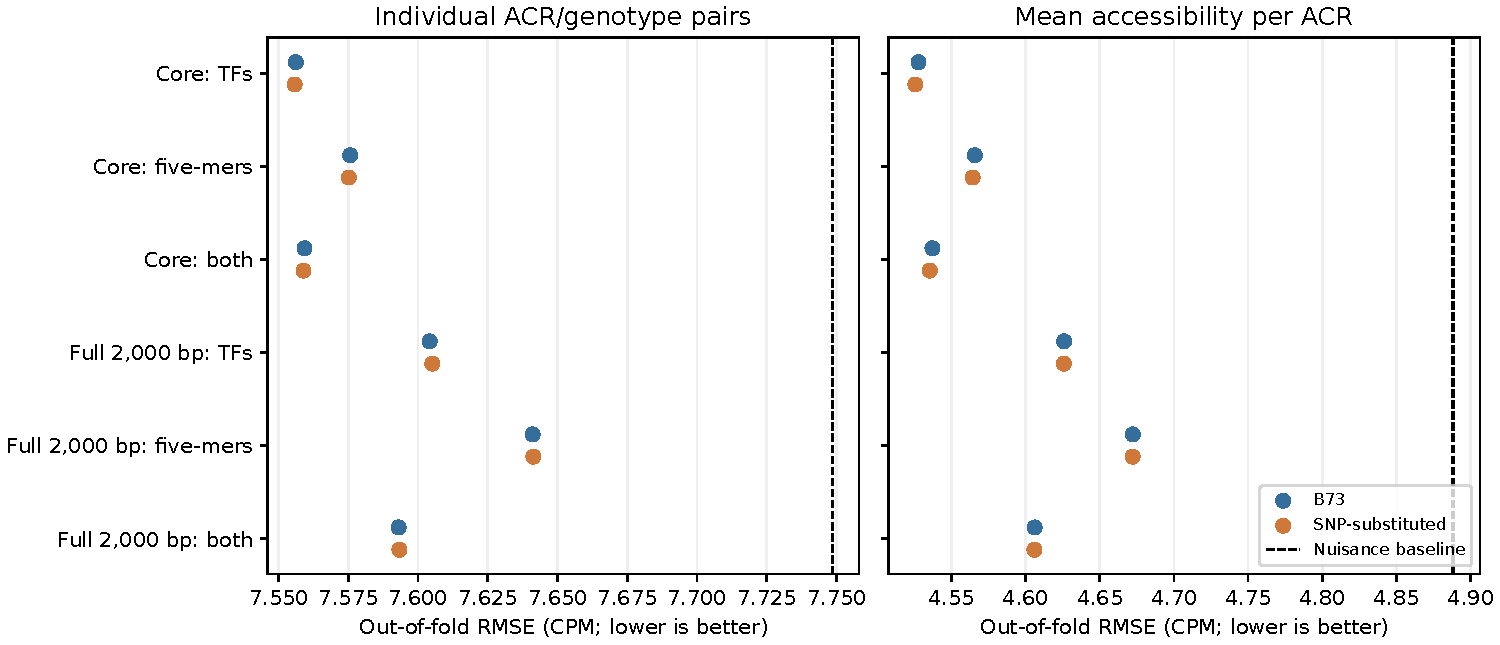
\includegraphics[width=\linewidth]{linear_comparison.pdf}
\caption{Matched linear predictions on held-out genomic blocks. Left: RMSE over all pairs; right: RMSE after averaging predictions and observations over the same available genotypes within each ACR. Dashed lines mark the nuisance baseline. TFs, 5-mer quasi-motifs, and their combination are compared for the core and full window using identical observations. Blue/orange distinguish B73 from SNP-substituted inputs; lower is better.}
\label{fig:linear}
\end{figure}

\subsection{Variation-rich subgroup evaluation}
I also evaluate the same globally trained models on the two sequence-variation-rich subgroups defined in Section~3.2. In the core-variation-rich group (2,167 ACRs; 70,594 pairs), baseline (nuisance covariates only) pair RMSE is 7.118805, versus 6.839241 for B73 core TFs and 6.838648 for personalized core TFs. In the context-variation-rich group (4,305 ACRs; 154,395 pairs), the corresponding values are 7.488848, 7.225135, and 7.224306. These within-subgroup comparisons again show little gain from personalization. 

Figure~\ref{fig:personalization} compares personalized inputs with the matched B73 model for every feature/extent combination. Positive values indicate lower squared error from personalization; their small magnitudes and mixed signs give no consistent predictive advantage. Even in these subgroups, within-ACR $R^2$ remains close to zero. Requiring multiple common reconstructed sequences therefore does not rescue genotype-level prediction with these linear scores.

\begin{figure}[htbp]
  \centering
  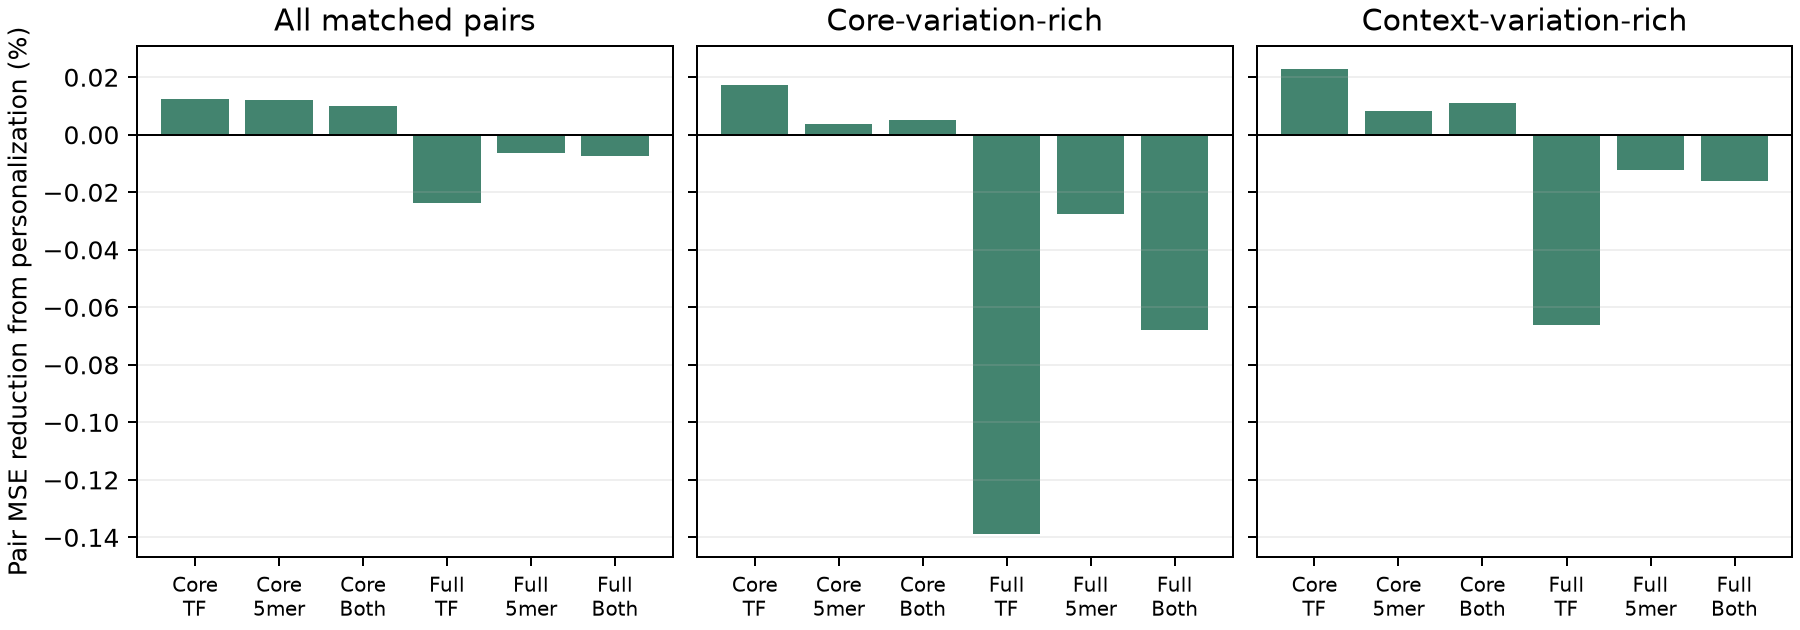
\includegraphics[width=\linewidth]{personalization_comparison.png}
  \caption{Change in pair MSE when substituting personalized for B73 inputs, calculated as $100(1-\mathrm{MSE}_{\mathrm{personalized}}/\mathrm{MSE}_{\mathrm{B73}})$ for the same model family and observations. Positive bars favor personalization.}
  \label{fig:personalization}
\end{figure}

\FloatBarrier

% Paste this subsection in place of the existing Section 5.3 placeholder.
% This is a section fragment, not a standalone LaTeX document.
% Upload both cnn_matched_comparison.pdf and cnn_earlier_comparison.pdf.
% The PNG versions show the same figures and are optional alternatives.
% Existing manuscript wording and the conclusion have not been changed.


\subsection{Matched CNN comparison}\label{sec:cnn-results}

I trained the four CNNs described in Section 4.3 using the same 9,666 qualifying ACRs and 495,900 (ACR, genotype) observations used to train the linear models and evaluated the CNN results using the same outer validation set metrics. Figure 5 shows the out-of-fold RMSE of the four CNNs versus the baseline covariate linear model and the two best-performing linear models which included the sequence statistics. The left panel shows RMSE weighting all (ACR, genotype) pairs equally, while the right panel shows RMSE of predicting average accessibility per ACR (so equally weighting ACRs and averaging their per-genotype predictions). Both panels tell a similar story: CNNs offer near identical validation set performance to the baseline linear model using only nuisance covariates. The differences in performance between the four model specifications are tiny as well, indicating negligible predictive advantage from using genotype-specific sequence versus reference or from using flanking sequence plus core versus the core sequence only. Forty-three of the 120 inner fits reached the 30-epoch limit, so this benchmark does not rule out better performance
with more extensive training.

Like the linear models, the CNNs which used genotype-specific sequence could explain almost none of the variance in accessibility between genotypes within fixed ACRs. This result suggests that, if there are generalizable sequence features whose disruption by SNPs causes differences in local accessibility, these CNNs are not able to capture them. Different architectures, training procedures, or larger training datasets may be able to predict changes in accessibility associated with SNPs, so this negative result is specific to the model architecture and training data I've employed here. 

I also include for comparison a smaller CNN which I had trained on the full set of (ACR, genotype) pairs. This smaller CNN uses reference sequence only and 2,048bp of context centered at the midpoint of each ACR. Architecturally, the smaller CNN divides its final sequence representation into eight consecutive segments and averages each of its 32 learned feature tracks within each segment. These
$8\times32=256$ values feed a fully connected prediction layer,
preserving coarse positional information instead of summarizing
each track only by its global mean and maximum. The earlier
network also receives an input channel identifying the original
ACR within the padded sequence. For each outer fold, I train
three networks with different random initializations, using the
same selected regularization strength and epoch budget, then
average their predictions. Each network has approximately 56,000
parameters, versus 144,000 in the four matched CNNs. The architecture and run settings of the smaller CNN are recorded in
\path{src/maize_regulatory/sequence_cnn.py} and
\path{results/sequence_cnn_benchmark/run_config.json}. To compare the smaller CNN with the larger models, I evaluated the earlier CNN's saved
outer-held-out predictions on exactly the same 495,900
ACR--genotype observations used in the matched experiment. The genomic-block fold
assignments agree, so every evaluated ACR was held out when
its prediction was generated. I mention this smaller CNN only because its performance on outer validation sets did represent a meaningful pickup versus all the models presented in the matched experiment ($R^2=0.319$ for average accessibility across ACRs, versus
$R^2=0.166$ for the best matched linear model). Figure 6 shows a comparison of mean accessibility $R^2$ across models, including this smaller CNN, as well as pair-weighted RMSE across folds. The performance across folds shows that in all five folds, the smaller CNN performs best, followed by the ridge model using TF motif scores on genotype-specific core sequence, and the larger CNN comes last. 



I have not performed further experiments to determine if the cause of the smaller architecture's outperformance is a larger training set (five-fold CV on all 108k ACRs instead of the ~10k available in the matched experiment), a more suitable architecture, or hyperparameter choices. What the comparison does establish is that there are potentially architectural or training limitations which are holding back the performance of the four main CNNs I outlined in 4.3. The earlier padded CNN nevertheless recovered additional predictive information about average accessibility
across ACRs, indicating that deep learning methods can improve on linear models but that improvement may be highly contingent on architecture and size of training dataset. 






\begin{figure}[htbp]
  \centering
  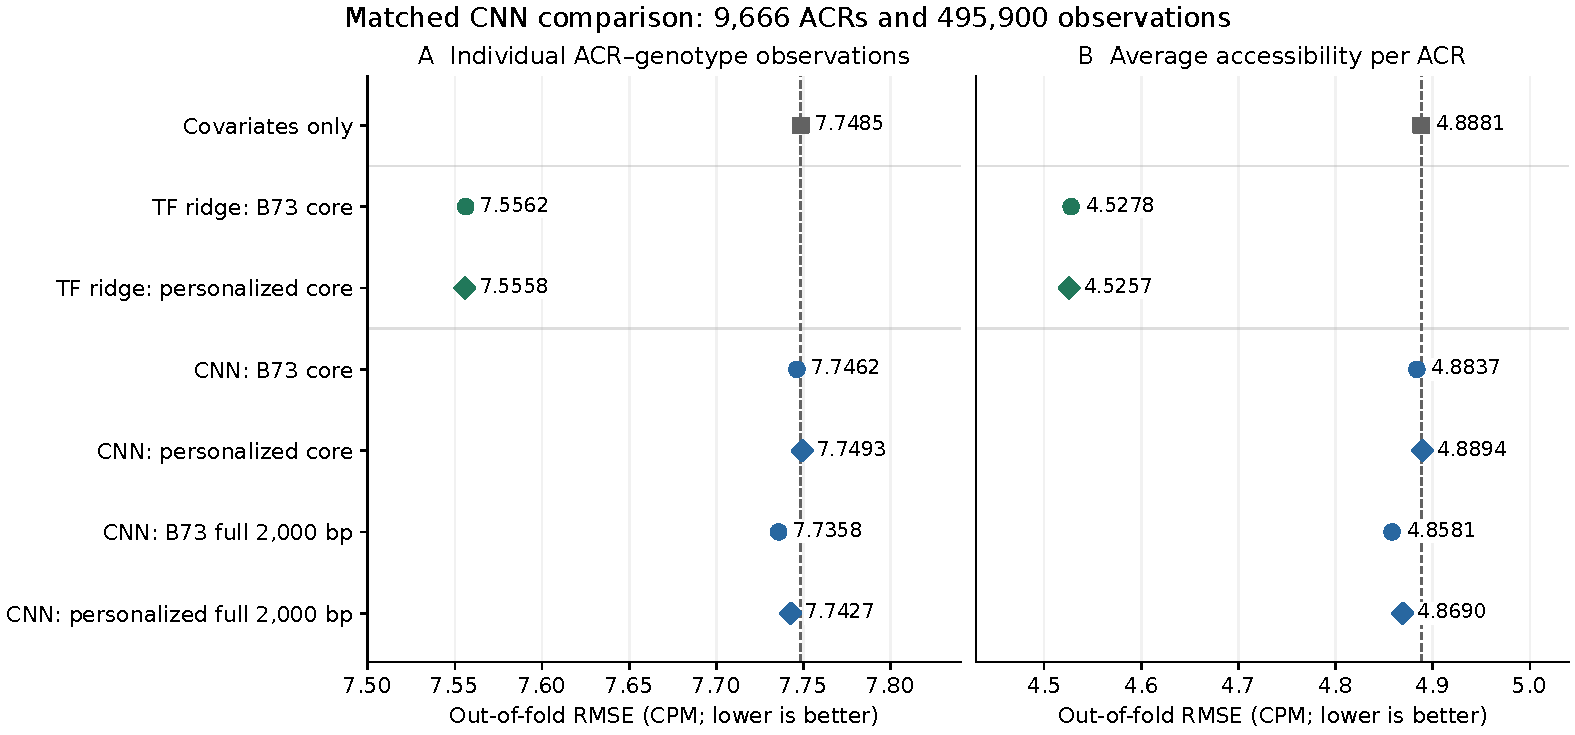
\includegraphics[width=\linewidth]{cnn_matched_comparison.pdf}
  \caption{Matched CNN and linear benchmarks on the same 495,900 ACR--genotype
  observations at 9,666 ACRs. Panel A scores predictions of individual
  ACR--genotype CPM values. Panel B first averages observed and predicted CPM
  over the same available genotypes within each ACR, then weights ACRs equally.
  Both panels show RMSE in CPM; lower is better. Dashed vertical lines mark
  the covariate-only baseline. All predictions come from the outer held-out
  genomic folds. The TF-ridge rows use core motif scores. The full-window
  CNNs use the entire centered 2,000-bp sequence. Axes are zoomed to show the
  observed differences; points are aggregate scores, not confidence intervals.}
  \label{fig:cnn-matched}
\end{figure}





\begin{figure}[htbp]
  \centering
  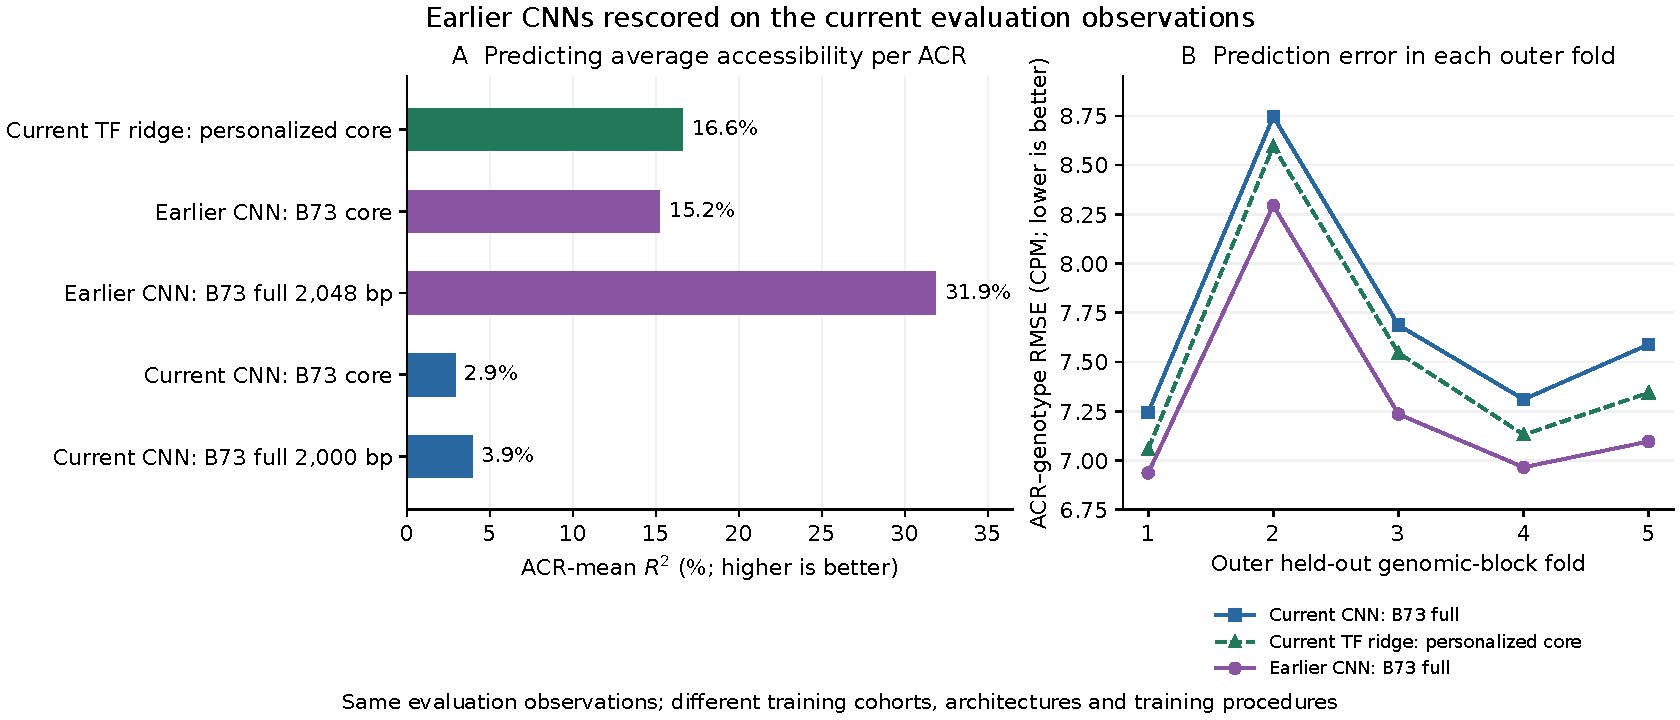
\includegraphics[width=\linewidth]{cnn_earlier_comparison.pdf}
  \caption{Earlier CNNs evaluated on the current 495,900 observations, using
  their saved predictions from the corresponding outer held-out genomic
  folds. Panel A shows $R^2$ for average accessibility across ACRs; higher is
  better. Panel B shows individual ACR--genotype RMSE in each outer fold;
  lower is better. Each point summarizes a different held-out group of genomic
  blocks. Fold numbers are categorical, and connecting lines identify models;
  these folds are not independent experimental replicates. Earlier models were
  trained using the larger catalog of 108,843 ACRs, whereas the current models
  use the 9,666 sampled ACRs. They also differ in architecture and training
  procedure. The earlier full window is 2,048 bp and the current full window
  is 2,000 bp. This comparison fixes evaluation observations, not training
  cohorts or sequence representations.}
  \label{fig:cnn-earlier}
\end{figure}





% ==================================================
\section{Conclusions, Limitations, and Future Directions}

My results show some predictive value in using sequence-based summary statistics as linear predictors of mean accessibility per ACR, while none of the models tested could recover meaningful variation between genotypes within ACRs. The baseline unpenalized regression using nuisance covariates only (length, GC content, chromosome, and ancestry proxies) had an $R^2$ of  0.0273 in predicting accessibility averaged across the available genotypes at each ACR. Linear models incorporating penalized motif scores and 5-mer scores had $R^2$ between $0.11$ and $0.17$. Larger sequence contexts slightly lagged the ACR-only models, while TF motif scores slightly outperformed the 5-mer quasi-motif scores. Overall, the differences between linear models using different levels of information were still quite small. Convolutional neural networks trained on the same ACR subset as the linear models performed about as well as the baseline nuisance regression, and like the linear models, could not predict differences in accessibility between genotype-specific sequences within ACRs. However, a smaller CNN trained via five-fold CV on all 108k ACRs using only reference sequence achieved a validation $R^2$ of $0.319$ on the matched experiment's dataset, suggesting that there may exist deep learning architectures and/or larger training sets which can surpass linear models at predicting average accessibility across regions. 

A few refinements might produce more successful deep learning models. Given that none of the tested models could explain much variance  between genotypes within the same ACR, there might be structural issues with representing genotype-specific sequence by substituting an incomplete SNP panel into B73. However, the current results do not distinguish incomplete
sequence representation from measurement variation between sequencing libraries (see Section 3.1), limited
sequence variation within ACRs, or limitations of the fitted
models and training procedures. A refined model might extend and tune my smaller CNN, which used reference sequence to predict accessibility averaged across the available genotypes at each ACR. This approach would enable training across more genomic regions, since the SNP substitution forced me to filter ACRs based on heterozygosity,  ambiguity, and number of available genotypes. As part of this extension, I would experiment with several candidate architectures and a larger grid of penalties; training was much more computationally expensive for the matched CNNs which incorporated genotype-specific sequence. If I scheduled this task on a compute cluster, training four or five candidate architectures across four or five candidate regularization strengths might be feasible. I would be curious to compare this more broadly trained and heavily tuned CNN to a hybrid architecture incorporating the sequence summary statistics which the linear models used. The first convolutional layer would be a predefined sliding log-likelihood-ratio calculation for a subset of TF motifs chosen by standardized effect size within training folds. By defining the first layer via TF motifs, we prespecify which short sequences the model should pay attention to but allow for the inner layers to discover more complicated sequence grammar. 

To improve the linear models, I am curious about adding richer, spatially informed grammatical features like sliding motif co-occurrence scores at specified offsets. This could balloon the feature set, so I would be open to considering only motifs implicated in the original Marand paper (TCP family) to create a manageable list of predictors for ridge to weight. 



% ==================================================
\begin{thebibliography}{9}
\bibitem{marand} Marand, A.~P., et al. (2025). The genetic architecture of cell type--specific cis regulation in maize. \textit{Science} 388, eads6601. \url{https://doi.org/10.1126/science.ads6601}. Pool memberships: Supplementary Data Table S2. Public ATAC data: \href{https://www.ncbi.nlm.nih.gov/geo/query/acc.cgi?acc=GSE273478}{GSE273478}; processed metadata: \url{https://doi.org/10.5061/dryad.nk98sf82v}.
\bibitem{jaspar} JASPAR 2026: expansion of transcription factor binding profiles and integration of deep learning models. \textit{Nucleic Acids Research}. \url{https://doi.org/10.1093/nar/gkaf1209}. Downloaded collection: 2026 CORE Plants, non-redundant PFMs.
\bibitem{reference} MaizeGDB. B73 reference genome, \texttt{Zm-B73-REFERENCE-NAM-5.0}. \url{https://download.maizegdb.org/Zm-B73-REFERENCE-NAM-5.0/}.
\bibitem{panzea} Panzea/MaizeGDB. B73-v5 282-panel chromosome-wise HapMap VCF distribution. \href{https://iastate.box.com/s/9edkm5f51q88ltzrb0hxaz4p36fdsr7q/folder/364949363629}{Public source folder}. Exact file identities and checksums are saved in the project input manifest.
\bibitem{hapmap} Bukowski, R., et al. (2018). Construction of the third-generation \textit{Zea mays} haplotype map. \textit{GigaScience} 7, gix134. \url{https://doi.org/10.1093/gigascience/gix134}. This describes the underlying HapMap resource; the particular v5 export used here is identified separately above.
\bibitem{tassel} TASSEL 5. Tutorial datasets: \texttt{mdp\_genotype.hmp.txt}, 3,093 SNPs on 281 maize association inbred lines. \url{https://tassel.maizegenetics.net/user_manual/appendix/tasseltutorialdatasets/}.
\end{thebibliography}

\appendix
\section{Supporting Analyses and Reproducibility}
The main comparison is the frozen matched sample, not the earlier experiments with different cohorts or response definitions. Earlier per-ACR local-SNP pilots asked whether variants predicted genotype differences at fixed regions, whereas the present global model asks whether sequence summaries predict accessibility at unseen regions. Neither a failure to improve prediction nor a descriptive library-variance comparison invalidates the source study's caQTL association results. Earlier reference-only CNN results use a different sample and 2,048-bp windows and are not inserted into the matched comparison.

The repository retains raw inputs separately from generated intermediates, frozen genotype/pair identifiers, sequence-pattern lookup tables, source/configuration hashes, fold manifests, selected penalties, fitted coefficients, and out-of-fold predictions. Identical sequences within an ACR are scored once and referenced through explicit genotype lookups. This avoids repeating sequence scans while preserving every actual pair in fitting. The selected scores contain 18,627 core patterns and 68,676 full-window patterns including B73 controls.

Numerical validation checked all 495,900 responses against raw pooled counts and whole-genome totals, all 8,960,382 selected B73 core TF scores against the existing score parquet (exact agreement), and independent direct motif/quasi-motif scans on sampled personalized sequences. All 60 sequence fits' explicit held-out pair errors agreed with their grouped cross-product calculations. Independent reconstruction of 2,080 saved predictions agreed within $8.9\times10^{-15}$ CPM, and four combined-feature training systems were checked with a separate linear-system solve. At benchmark completion, the Python suite had 163 passing tests and two Torch-dependent modules skipped in the primary environment. These checks reduce implementation risk but do not validate modeling assumptions or prove biological interpretation.

\begin{itemize}
\item Main numerical tables: \path{results/sampled_linear_benchmark/metrics.csv} and \path{fold_metrics.csv} in the same directory. Tuning and validation records are retained alongside them.
\item Sample and pair identities: \path{results/sampled_sequence_features/selected_acrs.parquet}, \path{pair_manifest.parquet}, and \path{feature_lookup.parquet} in that directory.
\item Variance definitions/results: \path{docs/cortex_cpm_variance.md} and \path{results/cortex_cpm_variance/}.
\item Scoring and fitting methods: \path{docs/sampled_sequence_features.md} and \path{docs/sampled_linear_benchmark.md}. Environment versions and input/code hashes are retained in the corresponding run receipts; the native numerical environment is pinned in \path{requirements-cnn-lock.txt}.
\item Report figures and the main LaTeX table are regenerated from existing outputs by \path{scripts/build_research_report_figures.py}; this does not refit any model.
\item CNN results: \path{results/sampled_cnn_benchmark/metrics.csv}.
The earlier CNN's saved held-out predictions, evaluated on the
current observations, are summarized in
\path{results/cnn_saved_prediction_comparison/metrics.csv}.
The checkpoint and split audit in
\path{results/cnn_saved_prediction_comparison/training_overlap_recheck.json}
confirms that every evaluated ACR was excluded from the training
set of the networks that generated its prediction.
\end{itemize}

\end{document}
